\documentclass{article}

\usepackage{polski}
\usepackage{graphicx}
\usepackage{listings}

\title{Optymalna gra w Monopoly}
\author{Dominik Wawrzyniuk}

\begin{document}

\maketitle

\section{Wstęp}

Projekt ma na celu analizę gry Monopoly metodami statystycznymi i teorii gier w celu zdefiniowania optymalnej strategii gry oraz weryfikacja tej strategii algorytmem maszynowym. Algorytm został wykonany w języku Python.

\section{Przyjęte zasady}

Analiza będzie odnosić się do konkretnych pól używając nazw angielskich załączonych na rysunku.

\begin{figure}
	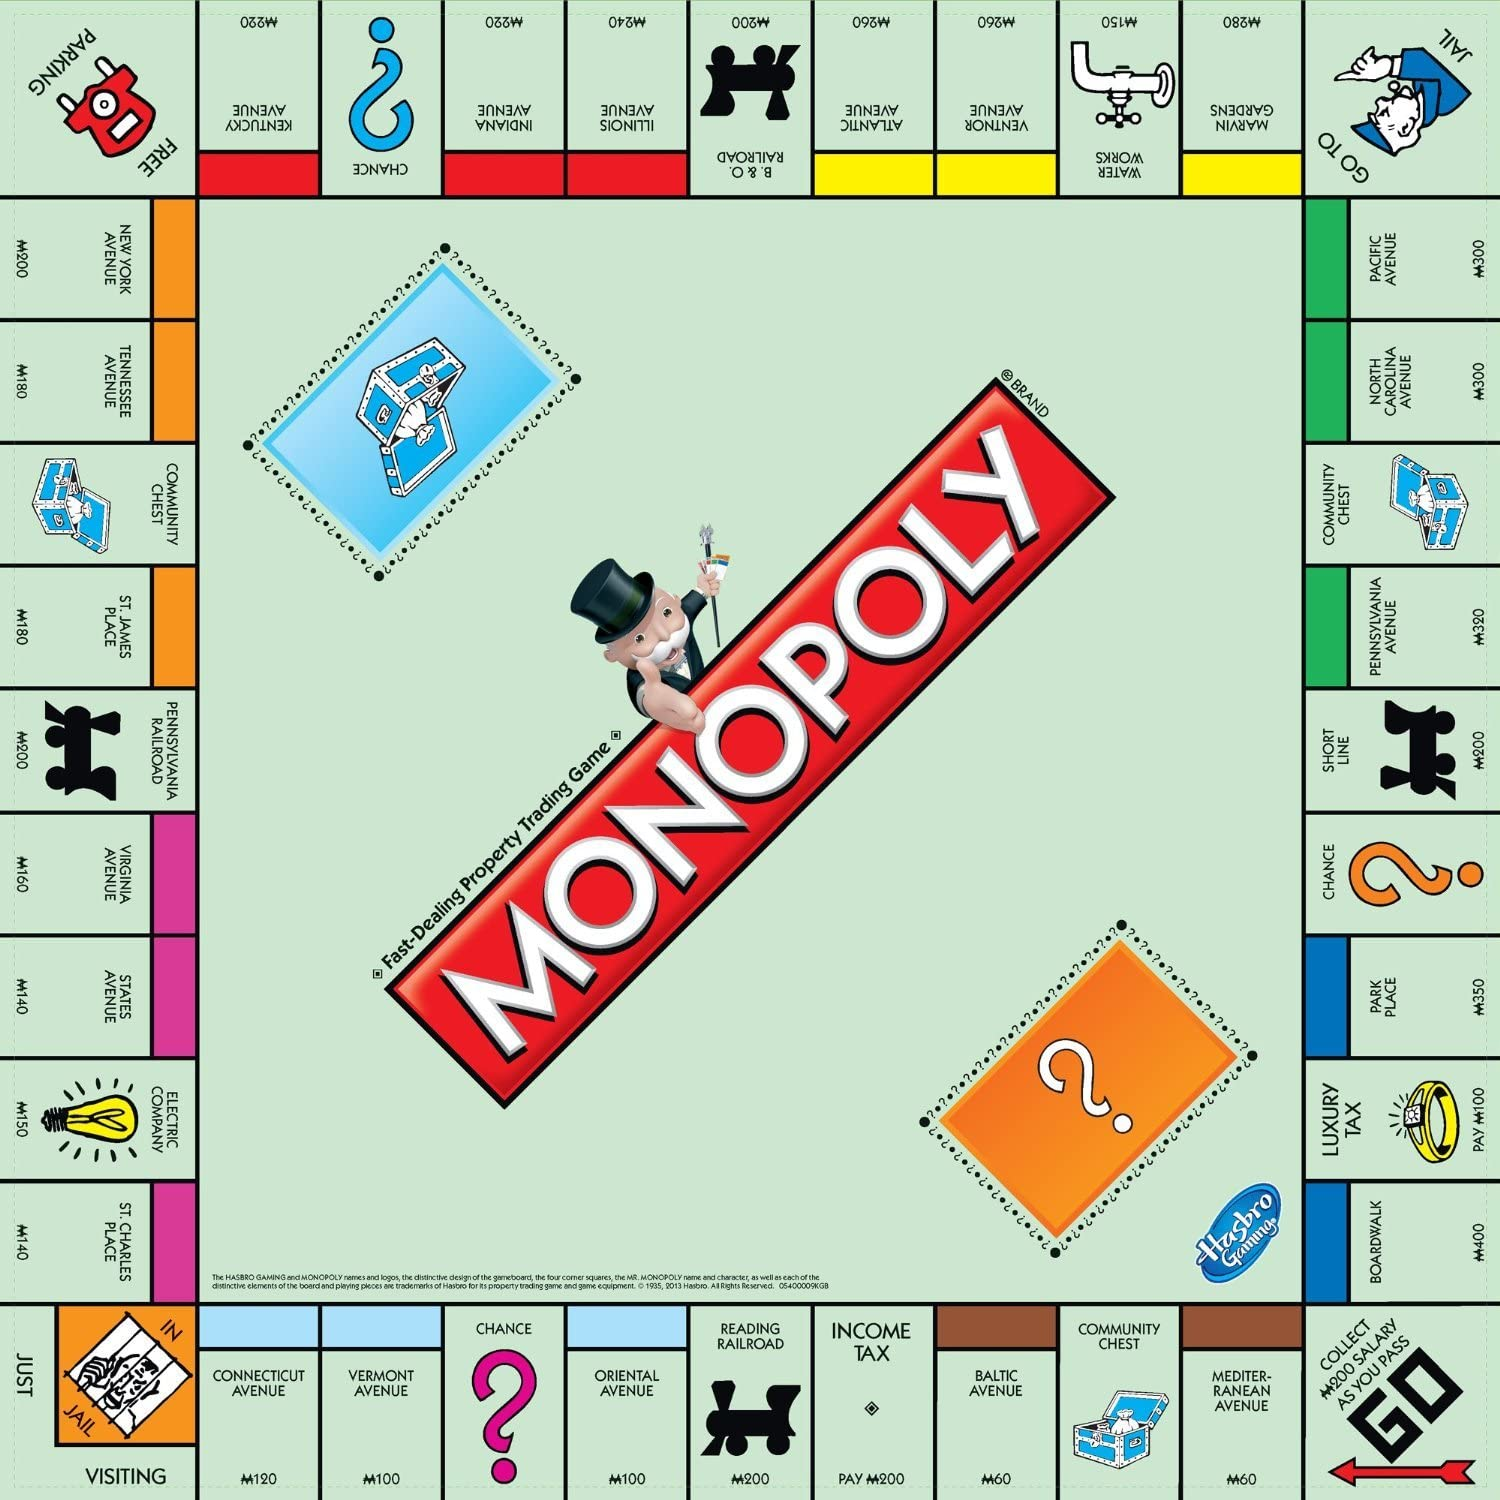
\includegraphics[width=\textwidth]{plansza}
	\caption{Plansza}
\end{figure}

Poniżej znajdują się strony, z których wzięte zostaną zasady na których bazować będzie niniejsza analiza.

\begin{itemize}
	\item Plansza: https://images-na.ssl-images-amazon.com/images/I/81btrHKgO0L.\_AC\_SL1500\_.jpg
	\item Zasady gry: https://www.hasbro.com/common/instruct/monins.pdf
	\item Ceny nieruchomości: https://monopoly.fandom.com/wiki/Property
	\item Karty szansy: https://monopoly.fandom.com/wiki/Chance
	\item Karty kasy społecznej: https://monopoly.fandom.com/wiki/Community\_Chest
\end{itemize}

\section{Zmiany zasad gry}

Zasady gry są przyjęte dokładnie takie same jak w załączonym pdf-ie z kilkoma zmianami.

\subsection{Koszty pola Income Tax}

Zniesiona zostanie opcja w której zamiast \$200 można zapłacić 10\% swojej wartości na polu Income Tax, ponieważ komputer potrafi policzyć swoją wartość w znacznie szybszym czasie od człowieka.

\subsection{Stała ilość domków i hoteli}

Ilość domków i hoteli nie będzie stała, ponieważ sytuacje w których miałoby znaczenie brak domków są marginalne i nie reprezentują dobrze typowej gry Monopoly. 

\subsection{Kara za niespłacenie hipoteki po kupnie}

Zniesiona jest zasada, w której kupując od gracza pole z hipoteką należy spłacić hipotekę od razu albo zapłacić dodatkowe 10 \% kwoty, ponieważ sytuacje te nie będą występować. Uzasadnienie tego w dalszej części sprawozdania.

\subsection{Oddanie pól graczowi winnemu bankructwa}

Zniesiona zostanie zasada, w której gracz po bankructwie musi oddać wszystkie swoje posiadłości graczowi winnemu tego bankructwa, ponieważ jest to zasada która potęguje efekt losowości i negatywnie wpływa na rezultaty testów.

\section{Reprezentacja gry}

\begin{figure}
	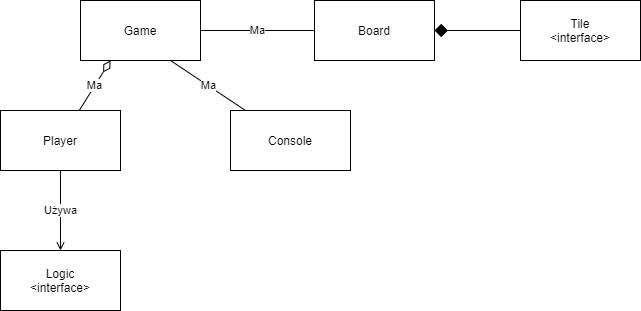
\includegraphics[width=\textwidth]{gra}
	\caption{Reprezentacja gry}
\end{figure}

\subsection{Game}

Klasa Game jest jedną instancją gry w Monopoly i przechowuje wszystkie informacje związane z tą konkretną grę. Jest ona odpowiedzialna za przekazywanie poleceń od klasy Player do klasy Console oraz odpowiadania na zapytania o np. pola albo graczy. Dodatkowo posiada metodę copy, która zwraca głęboką kopię danej instacji gry.

\subsection{Player}

Klasa Player reprezentuje gracza w grze. Używa ona interfejsu Logic w celu określenia działań podczas ruchu gracza, posiada on również odnośniki do pól które posiada oraz wszystkie inne informacje dotyczącego tego gracza takie jak ilość pieniędzy albo czy jest w więzieniu.

\subsection{Logic}

Interfejs Logic reprezentuje logikę za pomocą której gracz jest w stanie wykonać ruch. Działanie to jest realizowane metodą play. W ramach projektu zostały zaimplementowane dwa typy logiki; manualna i sztuczna.

\subsection{Console}

Klasa Console posiada określoną liczbę komend które jest w stanie wykonać. Komendy interpretowane są odpowiednim parserem poleceń. Klasa posiada kilka podklas realizujących konkretną rodzinę komend, m. in. TurnManager, który odpowiedzialny jest za zarządzanie przebiegiem tur w grze. Komendy przechowywane są w słowniku, z którego pobierane są metody.

\subsection{Board}

Klasa Board przechowuje listę wszystkich pól na planszy w danej grze. Pola reprezentowane są interfejsem Tile. Dodatkowo klasa posiada słownik pozwalający jej wiązać nazwy pól z ich pozycją na planszy. Posiada też metodę tworzącą planszę na podstawie danych zapisanych w plikach .json w katalogu data.

\subsection{Tile}

Interfejs Tile reprezentuje pole w grze. Istnieje wiele implementacji pól, między innymi pola Tax albo CardTile, dodatkowo istnieje oddzielny interfejs Property reprezentujący każde pole, które można kupić, również z kilkoma implementacjami. Interfejs Tile zawiera metody starting\_from\_event oraz landed\_on\_event, które definiują co się dzieje z graczem gdy zaczyna swój ruch z tego pola albo na nim ląduje.

\section{Realizacja logiki sztucznej}

Logika sztuczna składa się z kilku modułów, każdy odpowiedzialny za oddzielny element gry.

\subsection{MainLogic}

Klasa MainLogic jest główną implementacją interfejsu Logic. To on zawiera instancje wszystkich modułów oraz wiedzę o tym, w jakiej grze bierze udział i którym graczem steruje. Posiada on metody pozwalające na reakcję na cztery różne wydarzenia: decyzja odnośnie aukcji, decyzja odnośnie oferty handlowej, normalny ruch, ruch końcowy. MainLogic ma też metody pozwalające na podejmowanie decyzji odnośnie wychodzenia z więzienia za pomocą zapłaty grzywny bądź użycia karty. Dodatkowo zawiera parametr risk\_factor, definiujący chęć logiki do podejmowania ryzyka.

\subsection{SubLogic}

Interfejs SubLogic reprezentuje moduł służący do konkretnego elementu procesu decyzyjnego logiki sztucznej. Posiada on odnośnik do logiki, która go używa, oraz różne metody pozwalające uzyskać informacje odnośnie gry.

\section{Omówienie każdego modułu logicznego}

\subsection{AuctionLogic}

Ten moduł odpowiedzialny jest za podejmowanie decyzji dotyczących aukcji.

\subsubsection{Podstawy strategiczne}

W grze Monopoly posiadanie pól jest najważniejszą częścią gry. Żadne pole które nabędzie gracz nie jest bezużyteczne, ponieważ albo da nam dostęp do posiadania kiedyś całej tej grupy, albo da nam zasób za pomocą którego możemy dokonać handlu z kimś innym. Z tego też powodu powinniśmy zawsze kupować pole, jeżeli nas na nie stać. Przy takiej strategii aukcje stają się rzadkością. Mimo wszystko trzeba podjąć decyzje odnośnie kwoty jaką jesteśmy gotowi przeznaczyć na zwycięstwo w aukcji.

\subsubsection{Implementacja algorytmu}

Algorytm najpierw oblicza maksymalną kwotę, jaką jest gotowy poświęcić na aukcję. Wartość ta jest równa standardowej cenie pola pomnożonej przez współczynnik zależny od tego, czy my posiadamy wiele pól w danej grupie, albo inny gracz. Jeżeli aukcja toczy się o ostatnie pole w grupie, gdy pozostałe pola należą do jednego gracza, maksymalna kwota staje się ilością pieniędzy, jaką gracz posiada, ponieważ aukcja ta ma duże znaczenie dla przyszłości gry. Ilość pieniędzy które gracz jest gotowy zainwestować jest też zależna od chęci ryzyka gracza. Po obliczeniu maksymalnej kwoty algorytm podwyższa aktualną kwotę na aukcji o 1, dopóki to nie przekroczy maksymalnej kwoty albo wszystkich pieniędzy gracza.

\subsection{MortgageLogic}

Ten moduł odpowiedzialny jest za branie hipotek i sprzedawanie domków w celu utrzymania pozytywnej ilości pieniędzy gracza.

\subsubsection{Podstawy strategiczne}

Jeżeli gracz ma u kogoś długi, chcemy je spłacić minimalizując straty łącznej naszej szansy wygrania aktualnej gry. Dodatkowo zysk ze sprzedaży domku jest równy połowie ceny kupienia go ponownie, podczas gdy zysk wzięcia hipoteki jest równy ok. 90\% ceny spłaty hipoteki. Dlatego najpierw powinniśmy brać hipoteki na wszystkie pola które nie są częścią pełnej grupy którą posiadamy, potem sprzedawać domki w takiej kolejności, która minimalizuje straty zarobków, i ostatecznie wziąć hipoteki na pozostałe pola. Handlowanie z innymi graczami w celu wyjścia z długów omówione jest w dalszej części sprawozdania.

\subsubsection{Implementacja algorytmu}

Algorytm działa w pętli, która się powtarza dopóki gracz ma ujemną ilość pieniędzy. W pętli tej algorytm bierze hipoteki na pola, jeżeli ma pola bez wziętej hipoteki. Jeżeli nie ma, sprzedaje domek o najmniejszej wartości metody derivative, który równy jest stosunkowi straconego czynszu względem zysków ze sprzedaży. Jeżeli cała grupa nie ma już domków, algorytm bierze na nie hipoteki. Gdy nie ma już ani pól bez hipoteki, ani z domkami, algorytm kończy działanie i gracz przegrywa grę.

\subsection{TileLogic}

Ten moduł odpowiedzialny jest za budowanie domków oraz spłacanie hipotek.

\subsubsection{Podstawy strategiczne}

Decyzja, czy kupić domek, czy spłacić hipotekę, nie jest tak oczywista jak decyzja o wzięciu hipoteki lub sprzedania domku. Kupowanie domków zwiększa czynsz, jaki pobierzemy, zbliżając nas do wygranej. Spłacanie hipotek natomiast przywraca nam hipotekę, którą będziemy mogli kiedyś wziąć ponownie. Decyzja ta zależna jest od chęci gracza do ryzyka.

\subsubsection{Implementacja algorytmu}

Algorytm sprawdza, czy gracz posiada określoną ilość pieniędzy, zależną od chęci do ryzyka, zanim zacznie inwestować pieniądze w domki. Jeżeli tej kwoty nie ma, spłaca jedynie wszystkie hipoteki, które może.

\subsection{Wychodzenie z więzienia}

Wychodzenie z więzienia nie jest realizowane w oddzielnym module, a w klasie MainLogic. Odpowiedzialne jest za decyzję, czy warto wyjść z więzienia.

\subsubsection{Podstawy strategiczne}

Wychodzenie z więzienia jest korzystne wtedy, gdy jest względnie wiele pól bez właściciela, albo wtedy, gry możemy spodziewać się, że zarobimy cenę grzywny, albo więcej, podczas tur które byśmy w nim spędzili.

\subsubsection{Implementacja algorytmu}

Jeżeli wyjście z więzienia się opłaca, algorytm wyjdzie z niego albo kartą wyjdź z więzienia, jeżeli ją ma, albo płacąc kwotę, jeżeli ją ma. Opłacalność wyjścia może być potwierdzona jeżeli gracz uważa, że jest wystarczająco dużo pól bez właściciela, albo jeżeli zarobimy więcej niż zapłacimy. Ilość pieniędzy, jaką byśmy zarobili, jest aproksymowana.

\subsubsection{Aproksymacja zarobków poza więzieniem}

W Monopoly rzucamy dwoma kostkami z oczkami od 1 do 6. Wartość oczekiwana takiego rzutu to 7. Pól w Monopoly jest 40, więc podczas n ruchów jeden gracz okrąży całą planszę około

\begin{equation}
\frac{7}{40}n
\end{equation}

razy. Nasz łączny zarobek na okrążenie jednego gracza jest równy

\begin{equation}
	\frac{suma\_naszych\_czynszow}{40}
\end{equation}

przy założeniu, że szansa wylądowania na każdym polu jest równa. Założenie to jest błędne, co skutkuje błędem aproksymacji. W rzeczywistości każde pole ma inną szansę wylądowania, zależną od pozycji gracza. Na podstawie wyznaczonych zależności możemy aproksymować nasze zarobki w n turach wzorem

\begin{equation}
	ilosc\_graczy \cdot \frac{suma\_naszych\_czynszow}{40} \cdot \frac{7}{40}n.
\end{equation}

Od naszych potencjalnych zarobków musimy odjąć nasze potencjalne straty na okrążenie, które równe są

\begin{equation}
	\frac{suma\_strat}{40} \cdot \frac{7}{40}n.
\end{equation}

Jeżeli nasze potencjalne zarobki w turach, które byśmy spędzili w więzieniu, są równe lub większe od grzywny wyjścia z więzienia, to również warto z niego wyjść. Ostateczna aproksymacja zarobków poza więzieniem jest równa

\begin{equation}
	\frac{7n}{1600}\left(ilosc\_graczy \cdot suma\_naszych\_czynszow - suma\_strat\right).
\end{equation}

\subsection{TradingLogic}

Ten moduł jest odpowiedzialny za składanie innym graczom ofert handlowych. Jest on najbardziej obszernym modułem z własnym pakietem.

\subsubsection{Podstawy strategiczne}

Celem każdego handlu jest polepszenie własnej szansy na wygraną. Prawie wszystkie handle skutkują tym, że wszyscy uczestnicy handlu mają pod jego koniec jedną grupę na własność. Istnieją jednak inne rodzaje handli, które warto omówić. 
\paragraph{Handle ratujące gracza.}
Często w grach ludzkich dochodzi do sytuacji, w których jeden gracz ma dług u drugiego, i żeby gracz nie musiał sprzedawać domków ani brać hipotek, dokonuje handlu z drugim graczem dając mu pole w zamian za umorzenie długu. Taki handel jest niestety niepoprawny. Jeżeli gracz pierwszy po dokonaniu handlu nadal jest istotnym zagrożeniem dla drugiego gracza od względem wygrania gry, to niepowinien on się na taki handel zgodzić. Jeżeli po handlu natomiast gracz przestaje być zagrożeniem, to on się nie zgodzi, bo handel który obniża twoją szansę wygranej nie ma sensu. Dlatego moduł nie rozpatruje handli pola za pieniądze bez pól, ponieważ nigdy nie wystąpią one w optymalnej grze.
\paragraph{Handle Railroad i Utility.}
Innym rodzajem handlu jest handel polami typu Railroad albo Utility. Obie te grupy nie są na tyle korzystne dla właściciela, żeby chciał on mieć je na wyłączność, dlatego handlowanie tymi polami nie jest dla nikogo korzystne.
\paragraph{Dziedzina algorytmu.}
To zostawia jedynie handle z rodziny pole hotelowe za pole hotelowe i pieniądze. Handel taki musi albo dawać obu graczom możliwość przehandlowania tych pól później na pełne grupy, albo od razu im te grupy dawać. Należy wziąć dwie rzeczy pod uwagę.

Handlowanie 1 polem za 2 może być uczciwym handlem, pod warunkiem, że na koniec handli obie strony będą miały pełną grupę.

Jeżeli gracze znajdą handel skutkujący dla nich pełnymi grupami, istnieje kwota pieniężna, czyniąca ten handel uczciwym. Gdyby istniała w grze możliwość zagwarantowania, że gracz nigdy nie będzie musiał zapłacić czynszu na danym polu, możliwe byłyby idealnie uczciwe handle, ponieważ żadna strona nic nie traci, a jedynie zyskuje. Niestety nie ma takiej możliwości, ale podczas gry gracz straci określoną kwotę pieniężną na polach drugiego gracza. Jeżeli gracz dostałby tą kwotę odgórnie od tego drugiego gracza, obie strony miałyby równą szansę wygranej.

\subsubsection{Implementacja algorytmu}

Algorytm składa się z kilku części. Posiada on tłumacz wyniku algorytmu na polecenia dla klasy Console, metody pozwalające doprowadzić dane do postaci obsługiwanej przez algorytm, oraz liczne klasy potrzebne do poprawnego działania algorytmu.
\paragraph{Notacja.}
Grupy pól reprezentowane są w postaci ciągu identyfikatorów właścicieli. Przykładowo grupa trzech pól, gdzie pierwsze i trzecie należą do gracza 0, a drugie do gracza 2, byłoby zapisane jako 020.
\paragraph{Krok 0: Dane wejściowe}
Punkt wejściowy algorytmu to metoda solve\_for w klasie Trader. Algorytm w postaci teoretycznej dostaje na wejście jedynie ciąg grup, np. 002 112 324 304 304 oraz gracza dla którego szukamy handlu, i ma on zwrócić możliwy handel dla danego gracza. W implementacji algorytm dostaje również klasę MoneyCalculator, aby zweryfikować, czy gracze mają wymagane kwoty do handlu.
\paragraph{Krok 1: Możliwe rozwiązania}
Ten krok dzieje się w klasie Combiner. Iterując po grupach, sprawdza on, kto musiałby wziąć udział w handlu, aby ta grupa mogła należeć do gracza. Następnie rekursywnie sprawdza on dla każdego gracza w handlu pozostałe grupy.
Przykład działania w pliku krok1.txt.
W powyższym przykładzie tracimy informację odnośnie tego które pola faktycznie kto potrzebuje, ale implementacja przechowuje te dane. Algorytm znajdzie wszystkie takie możliwe rozwiązania. Na koniec sortuje on je względem ilości graczy, którzy muszą wziąć udział w handlu. Im mniej tych graczy, tym lepszy handel dla jego uczestników. Handel, w którym wszyscy gracze biorą udział, nic nikomu nie daje, dlatego teoretycznie algorytm nie powinien brać takich handli pod uwagę. Niestety bez takich handli gry potrafią się dłużyć i zbiegać do remisów, dlatego w implementacji zostały dopuszczone wszystkie handle.
\paragraph{Krok 2: Zbuduj graf}
Ten krok odbywa się również w klasie Combiner, równolegle z krokiem 1. Na podstawie otrzymanego rozwiązania zbuduj graf potrzeb, w którym każdy gracz jest węzłem posiadającym krawędź skierowaną do węzłów, które posiadają pola w grupie przeznaczonej danemu graczowi.
Przykład działania w pliku krok2.txt.
\begin{figure}
	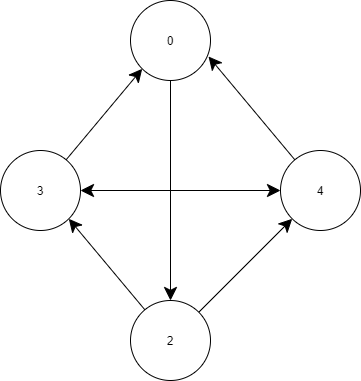
\includegraphics[width=\textwidth]{graf}
	\caption{Graf potrzeb}
\end{figure}
\paragraph{Krok 3: Przejdź przez graf}
Ten krok dzieje się w klasie Walker. Nazwijmy gracza, dla którego chcemy znaleźć handel celem, a gracza, do którego cel ma dostęp startem. Algorytm zaczyna z dowolnego startu i znajduje każdą ścieżkę która prowadzi z powrotem do węzła naszego gracza. Następnie powtarza on tą czynność z celu, nie przechodząc przez węzeł użytego startu. Każdy węzeł, z którego dotarliśmy zaczynając ze startu, ale nie z celu, musimy przehandlować z graczem którego reprezentuje start. Algorytm powtarza tą czynność dla każdego startu.
\paragraph{Krok 4: Znajdź kwotę pieniężną}
Ten krok odbywa się w klasie MoneyCalculator. Aktualnie zaimplementowany został algorytm, który każe każdemu graczu zapłacić drugiemu 1\% różnicy ich czynszów, gdy będą mieli hotele. Te wartości są bardzo małe, prawie równe zeru. Niestety, przy większych wartościach kwoty są na tyle duże, że prawie nigdy nie dochodzi do handli.

\section{Rezultaty testów}

\subsection{Symulacje Monte Carlo}

W wielu miejscach, np. w kwocie aukcji albo kwocie handlu, symulacje Monte Carlo pozwoliłyby otrzymać lepszą wartość kwoty pieniężnej, która daje obu graczom wzrost szansy wygranej. Niestety jedna taka symulacja zajmuje średnio 0.17 sekund, co jest zbyt długim czasem aby wykonać tych symulacji na tyle, żeby mieć wystarczająco dobry wynik. Dlatego w miejscach, gdzie miałby on zastosowanie, użyto aproksymacji.

\subsection{Remisy}

Niektóre gry trwają dłużej od innych, ponieważ czasem gracze nie są chętni do podejmowania ryzyk, co sprawia, że bardzo powoli tracą pieniądze, albo nie tracą ich wcale. Usunięcie limitu uczestników w handlu oraz zmniejszenie kwot handli znacznie zmniejszyło czas średniej gry oraz występowanie takich sytuacji.

\subsection{Chęć podejmowania ryzyka a zwycięstwo}
Wyniki znajdują się w pliku results.txt. Najczęściej wygrywają gracze z wartością risk\_factor z zakresu (0.8, 1),  a najrzadziej (0, 0.2). Warto więc podejmować ryzyka.


\end{document}